\documentclass[handout]{beamer}
\usepackage{array}
\usepackage{german}
\usepackage{graphicx}
\usepackage[utf8]{inputenc}
\usepackage[T1]{fontenc}
\mode<beamer>{%
\usetheme{Copenhagen}
}
\usepackage[orientation=landscape,size=a3,debug,scale=2.5]{beamerposter}
\title[]{}
\begin{document}
\begin{frame}
\frametitle{%\hspace{0pt plus 1 filll}
MathSem 2024: Variationsprinzipien}
\begin{columns}[t,onlytextwidth]
\begin{column}{0.32\textwidth}
\begin{center}
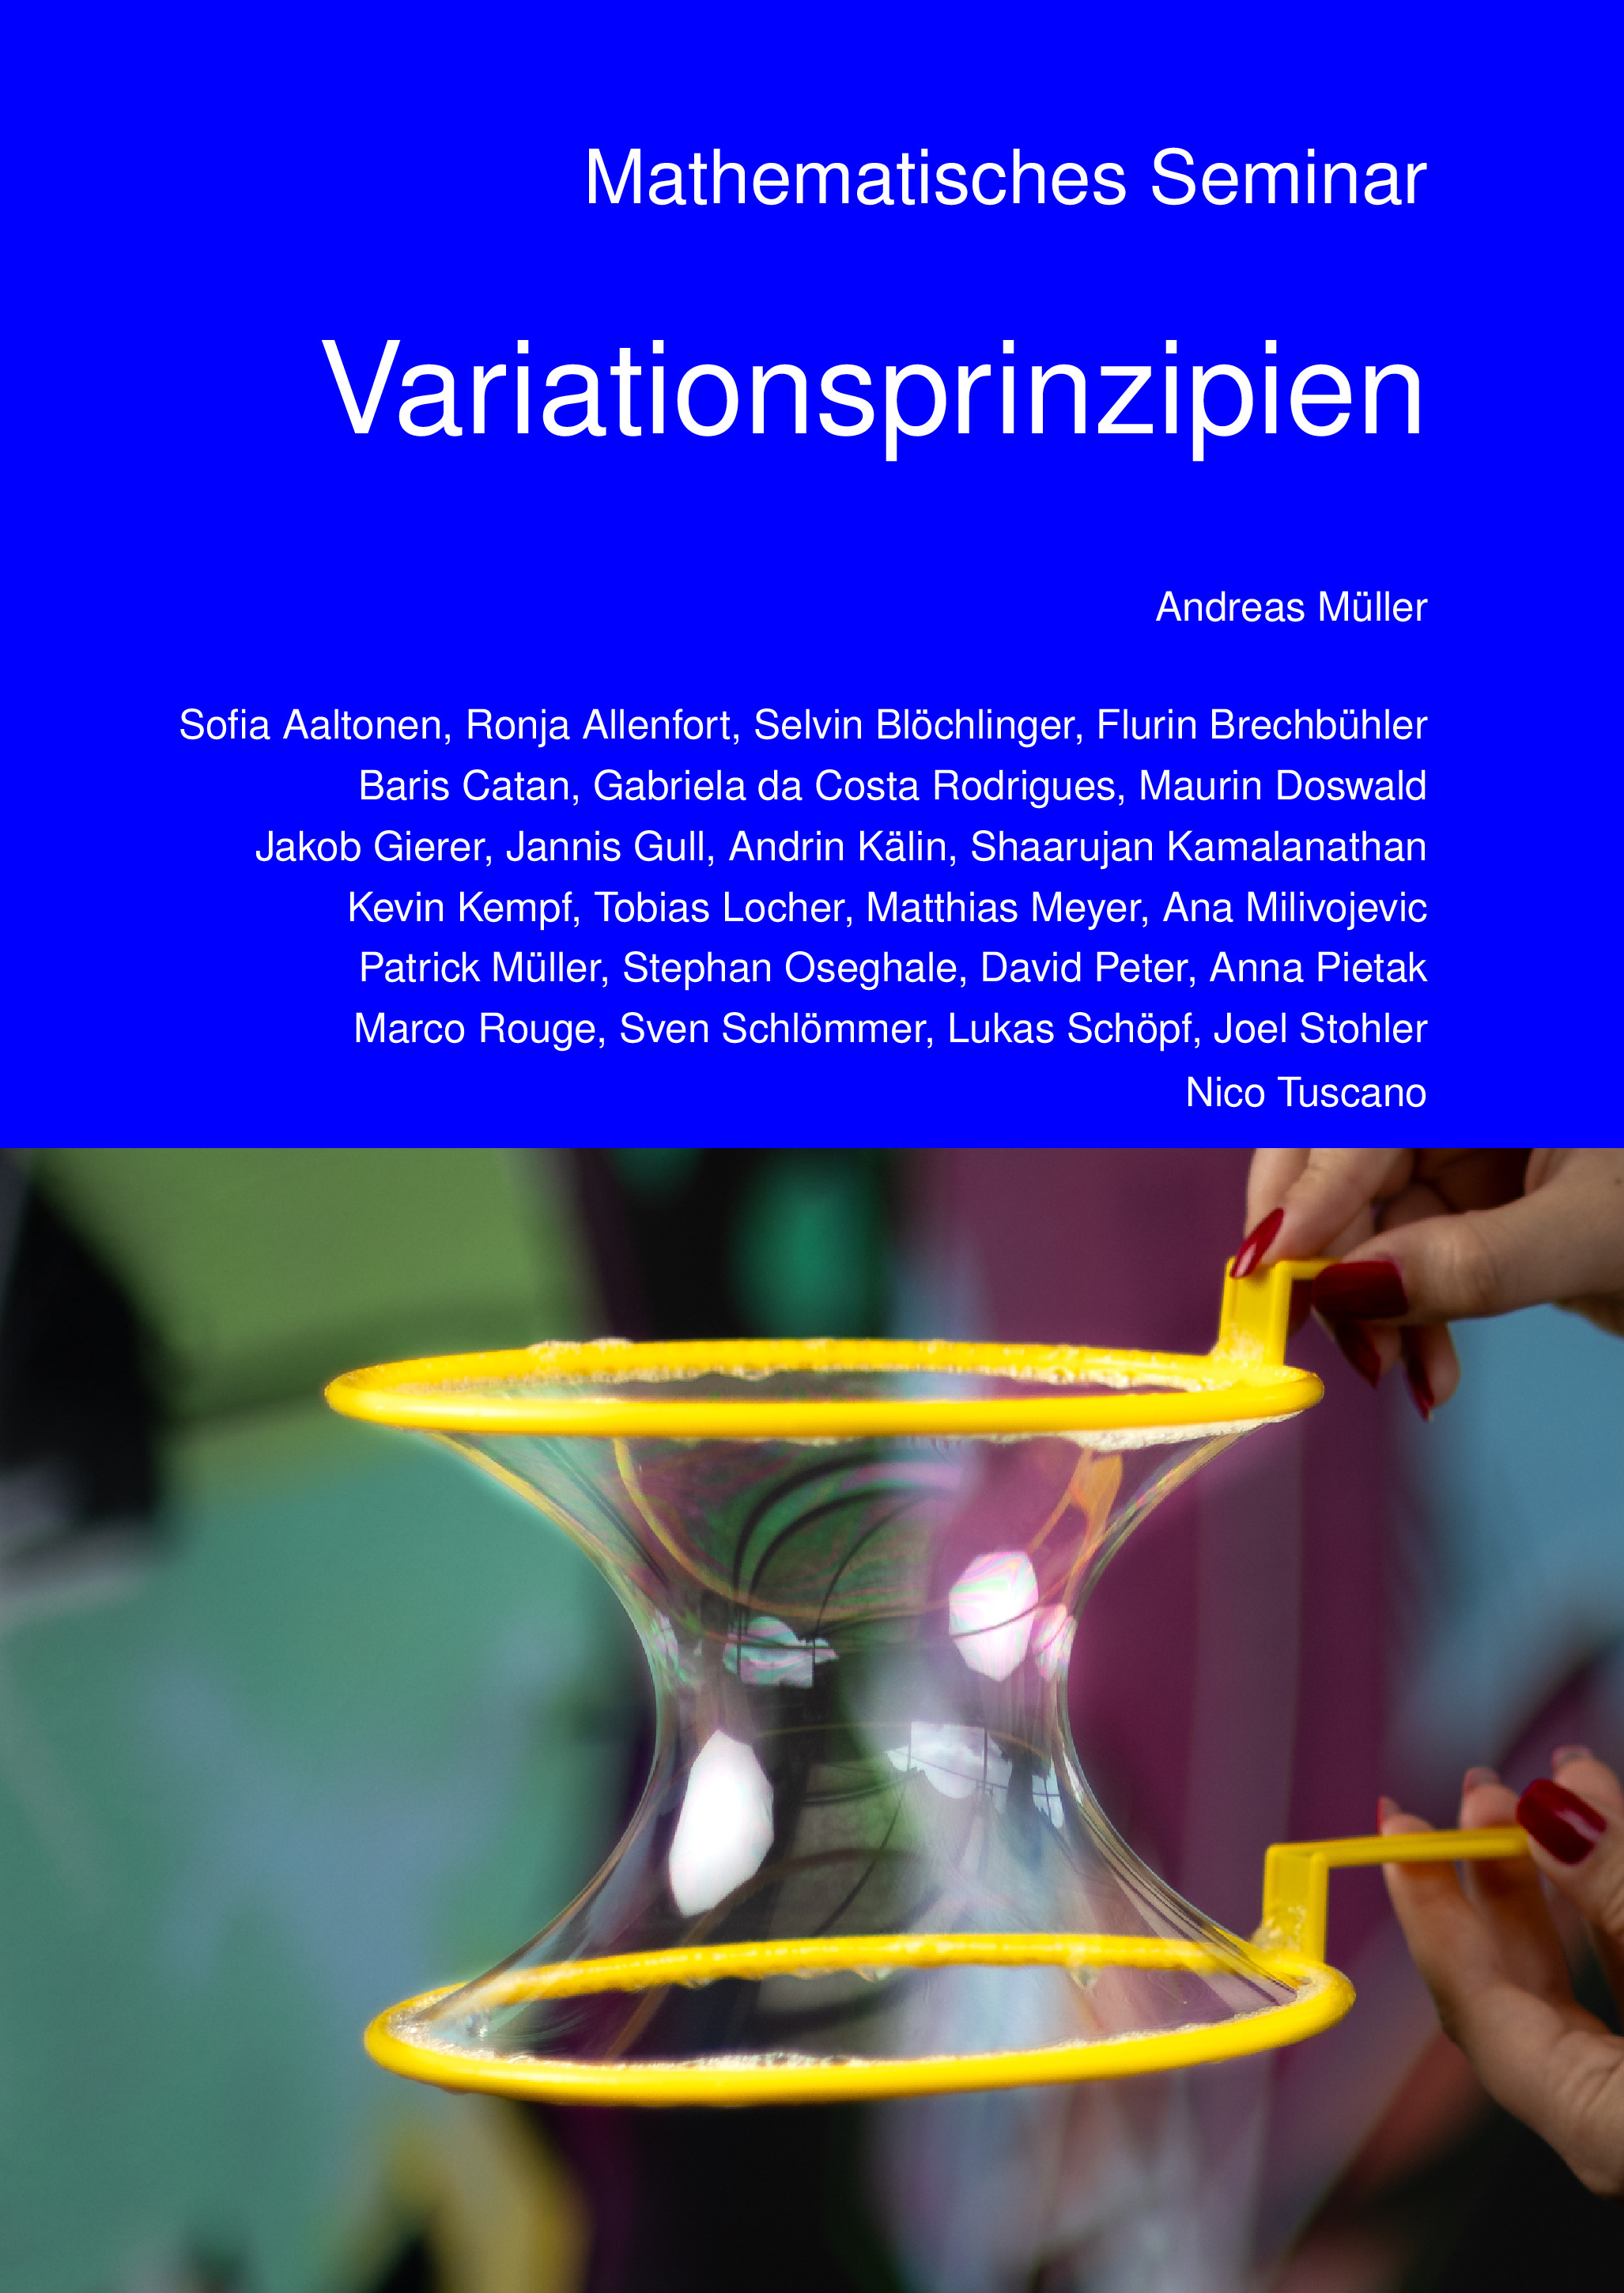
\includegraphics[width=\hsize]{../cover/buchcover.png}
\end{center}
\vskip 0.2cm
\bigskip
\bigskip
Erscheint~im~Herbst~2024.\\
Anfragen~an~Prof.~Dr.~Andreas Müller,\\
{\texttt{andreas.mueller@ost.ch}}
\bigskip
\bigskip
\bigskip
%\vskip 1.2cm
\end{column}
%
\begin{column}{0.65\textwidth}
\begin{description}
\item[Teil 1:] Grundlagen
\begin{enumerate}
\item Extremalprobleme für Funktionen mehrere Variablen
\item Erste Variation
\item Nicht differenzierbare Lösungen
\item Variationsprinzipien für Felder
\item Variationsprobleme mit Nebenbedingungen
\item Zweite Variation
\item Direkte Methoden
\item Hamilton-Jacobi-Theorie
\item Klassische Mechanik
\item Symmetrien
\end{enumerate}
\item[Teil 2:] Anwendungen und weiterführende Themen
\begin{enumerate}
\setcounter{enumi}{10}
\item Shaarujan Kamalanathan: {\em Doppelpendel}
\item Tobias Locher und Nico Tuscano: {\em Kettenlinie}
\item Ronja Allenfort und Ana Milivojevic: {\em Minimalflächen}
\item Sofia Aaltonen und Gabriela Rodrigues: {\em Balkengleichung}
\item Sven Schlömmer: {\em Oberflächenwasserwellen}
\item Selvin Blöchlinger: {\em Relativistische Mechanik}
\item Maurin Doswald und Stephan Oseghale: {\em Maxwell-Gleichungen}
\item Andrin Kälin und Marco Rouge: {\em Geodäten}
\item Matthias Meyer: {\em Elektrische Schaltungen}
\item Baris Catan und Jannis Gull: {\em Antennen}
\item Flurin Brechbühler: {\em Finite Elemente}
\item Anna Pietak: {\em Die optimale Flussüberquerung}
\item David Peter und Joel D. Stohler: {\em Raketenflugbahn in einen Orbit}
\item Jakobi Gierer und Lukas Schöpf: {\em Warum sind Planeten Sphären?}
\item Kevin Kempf: {\em Variationsprinzipien für Algorithmen}
\item Patrick Müller: {\em Cahn-Hilliard-Gleichung}
%\item Andreas Müller: {\em Die newtonsche Widerstandsformel}
\end{enumerate}
\end{description}
\end{column}
\begin{column}{0.01\textwidth}
\llap{\raisebox{-3cm}{\includegraphics{qrcode.pdf}}}
\end{column}
\end{columns}
\end{frame}
\end{document}
